\chapter{Algoritmy na grafoch}
\label{kap:algoritmy}

Táto kapitola obsahuje popisy algoritmov, ktoré sú aplikovateľné na grafové štruktúry a navyše využiteľné pri vyhľadávaní spojení hromadnej dopravy. Formálnu charakterizáciu algoritmu zväčša doprevádza i jeho voľnejšia interpretácia, ktorá má za účel uľahčiť porozumenie čitateľom, ktorí sa s daným algoritmom doposiaľ nestretli. Naviac, pri algoritmoch sú uvedené výhody, respektíve nedostatky, pri jeho použití na nami vytýčený cieľ. V hojnom počte budeme využívať definície z kapitoly \ref{kap:grafy}.\newline


\section{Prechádzanie vrcholmi grafu}

Stručne popíšeme základné algoritmy na prechádzanie vrholov grafu. Tie však nie sú priveľmi využiteľné pri vyhľadávaní spojení MHD. Môžu nám ale významne pomôcť k prechádzaniu objemných súborov dát, ktoré bude sieť hromadnej dopravy isto obsahovať.\newline


\subsection{Prehľadávanie do šírky}

Prehľadávanie do šírky alebo skrátene BFS (z anglického Breadth-first search), dokáže pejsť cez všetky vrcholy grafu zapomoci fronty (alebo radu). Algoritmus si do nej ukladá susedov spracúvaných vrcholov, a tak prehľadá celý graf, pričom v každej iterácií prejde o jednu hranu viac vzdialené vrcholy od počiatočného.\newline

\begin{figure}[H]
  \centering{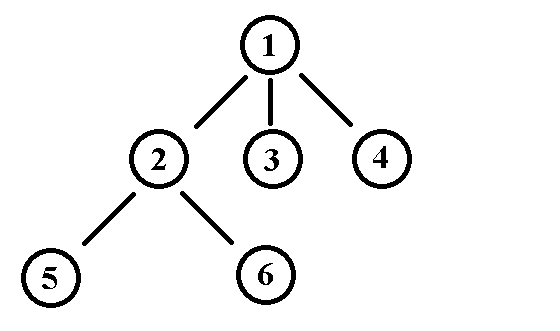
\includegraphics{./images/BFS_priklad.png}}
  \caption{Príklad práce BFS na strome}
  \label{BFS_priklad}
\end{figure}


\subsection{Prehľadávanie do hĺbky}

Prehľadávanie do hĺbky, skrátene DFS (z anglického Depth-first search), prechádza cez vrcholy grafu len pomocou cyklu, prípadne rekurzie. Obvykle sa v algoritme na všetkých susedov vrchola zavolá postupne rekuzívne ten istý algoritmus prehľadávania.\newline

\begin{figure}[H]
  \centering{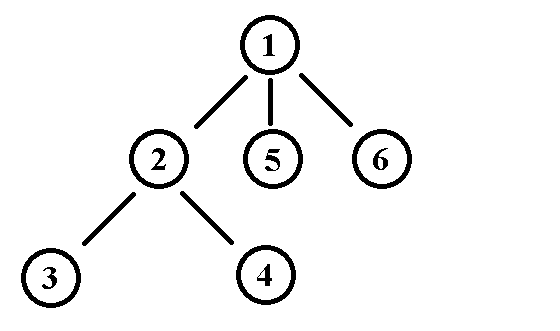
\includegraphics{./images/DFS_priklad.png}}
  \caption{Príklad práce DFS na strome}
  \label{DFS_priklad}
\end{figure}

Je vhodné poznamenať, že na pbrázku~\ref{DFS_priklad} je ukázané len jedno z možných poradí práce s vrcholmi. Samozrejme, vrcholy budú vždy navštívené vo vyobrazenom poradí, avšak práca s nimi môže byť vykonaná až tromi spôsobmi. Prvý z nich súhlasí s usporiadaním na obrázku a nazýva sa \textit{preorder}. Ďalšie dva sú \textit{inorder} a \textit{postorder}.\newline


\subsection{Zhrnutie}

Obi dva algoritmy majú očividnú lineárnu časovú zložitosť ($O(n)$), nakoľko sa pozrú na každý vrchol grafu práve raz.\newline

Ako sme už spomínali, v týchto algoritmoch nevidíme potenciál pri ich využití na uskutočnenie nášho cieľa. Ich znalosť však môže byť veľmi prínosná pri prechádzaní štruktúr našich grafov.\newline


\section{Najlacnejšie cesty v grafe}

Pri vyhľadávaní spojení mestskou hromadnou dopravou sa zdá byť veľmi racionálne zaoberať sa nachádzaním najlacnejších ciest v grafikone MHD. Dovoľujeme si tak tvrdiť, pretože najväčší dôraz cestujúcich je kladený práve na čo najskorší príchod do požadovanej lokality. Pre úplnosť ešte dodávame, že cena cesty, ako je asi zrejmé, je súčet hodnôt hrán (respektíve vrcholov), ktoré daná cesta obsahuje. Z doposiaľ uvedeného vyplýva, že pri našich úvahách budeme používať ohodnotené grafy, kde pridelenou hodnotou bude čas medzi zastávkami. Navyše musíme nejako ošetriť i vrcholy grafu - zastávky, keďže na nich zvyčajne čakáme na prestup na ďalší spoj. Od tejto myšlienky však spočiatku upustíme a budeme sa jej venovať až neskôr. A posledná úvaha - hranami v našom grafe sú linky MHD, sme preto nútení použiť orientované grafy.\newline

Ak uvažujeme vyhľadávanie najlacnejších ciest v grafe, musíme si najprv uvedomiť, čo presne je našim cieľom. Výledok, ktorý chceme dosiahnuť ako výstp algoritmu, má byť najlacnejšia cesta z počiatočného bodu do koncového. Avšak znalosť problematiky algoritmov na grafových štruktúrach nám ponúka riešenia iného, koplexnejšieho problému s asymptoticky rovnakou časovou zložitosťou. Týmto problémom je vyhľadávanie najlacnejších ciest z počiatočného vrcholu do všetkých ostatných vrcholov. Ľahko nahliadnuť, že riešeim tohto problému dostaneme odpoveď aj na našu počiatočnú otázku.  Preto sa v nasledujúcej časti budeme zaoberať algoritmami riešiacimi túto úlohu.\newline

Ľahko spozorovať, že by mohlo byť v určitých situáciách výhodné vypočítať ceny a nájsť najlacnejšie cesty pre všetky dvojice vrcholov. Hlavne, keď graf obsahuje malé množstvo vrcholov - zastávok. Mnoho miest má len malú sieť mestskej hromadnej dopravy, a teda by bolo rozumné vypočítať všetky potrebné údaje naraz na začiatku, a potom, pri prijímaní dotazu na vyhľadanie spojenia, jednoducho vypísať už vypočítanú odpoveď. Z tohto dôvodu uvedieme i algoritmy riešiace tento problém.\newline


\subsection{Dijkstrov algoritmus}
\label{Dijkstra}

Holandský informatik, po ktorom je tento algoritmus pomenovaný, dokázal, okrem iného, vyriešiť aj nami nastolený problém. V jeho riešení je ale potrebné, aby boli ceny hrán grafu nezáporné reálne čísla, čo súhlasí s našou predstavou aplikovania algoritmu na grafikon MDH. Algoritmus je navrhnutý tak, že dostane ako vstup graf $G = (V, E)$, počiatočný vrchol $v_{0}$ a hodnotiacu funkciu $h: V \times V \rightarrow R^{+}_{0}$. Predpokladáme, že ak hrana $uv \notin E$, potom $h(u,v) = \infty$, ďalej, že $h(u,u) = 0$ a nakoniec, že funkciu $h$ je možné vypočítať v konštantnom čase $O(1)$. Máme taktiež jeden predpoklad na vrcholy grafu, a to, že sú reprezentované celými číslami $1, 2, ... , k$ (kde $k$ je počet vrcholov grafu). Nakoniec, výsledkom algoritmu bude pole čísel $D$, v ktorom bude pre každý vrchol $v \in V$ vypočítaná hodnota $D [v]$, čo je cena najlacnejšej cesty z počiatočného vrchola $v_{0}$ do vrchola $v$.\newline

Tieto požiadavky, predpoklady, ba i vstup a výstup funkcie sú uvažované v horeuvedenom tvare len aby sme mohli predviesť implementáciu algoritmu od Pavla Ďuriša, ktorú možno nájsť aj v jeho knihe \cite[kapitola 2.2.1]{duris2009}.\newline

\begin{algorithm}[H]
  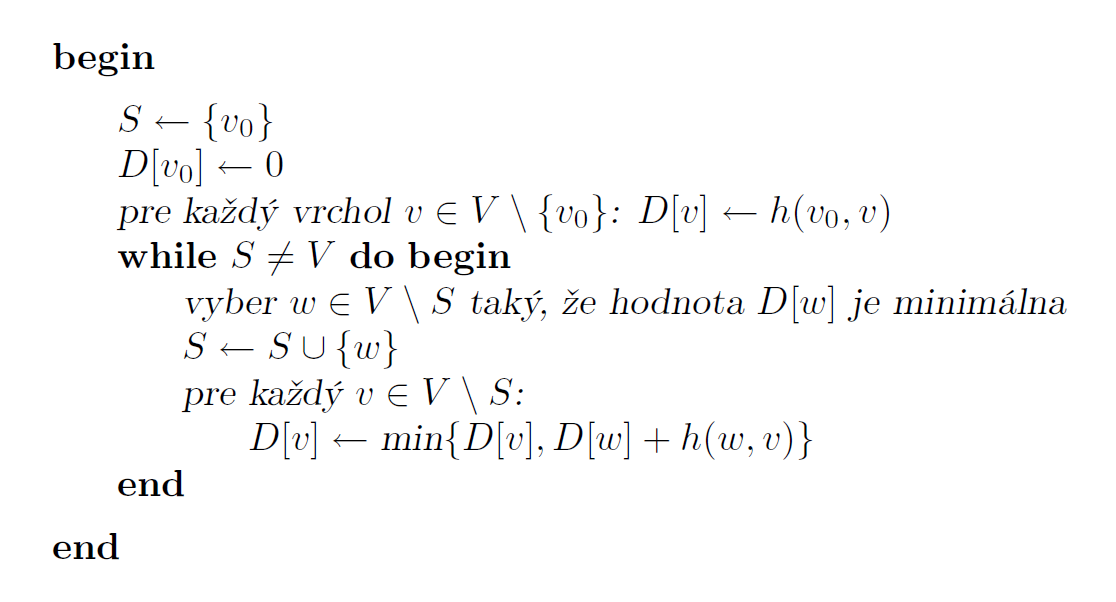
\includegraphics[width=\linewidth]{./images/Alg_Dijkstra.png}
  \caption{Dijkstrov algoritmus}
  \label{Alg_Dijkstra}
  \centering
\end{algorithm}

Časová zložitosť dijkstrovho algoritmu je $O(|V|^{2})$, čo je dokázané spolu s jeho korektnosťou v už uvedenom zdroji od Pavla Ďuriša \cite[kapitola 2.2.1]{duris2009}.\newline

\begin{figure}[H]
  \centering{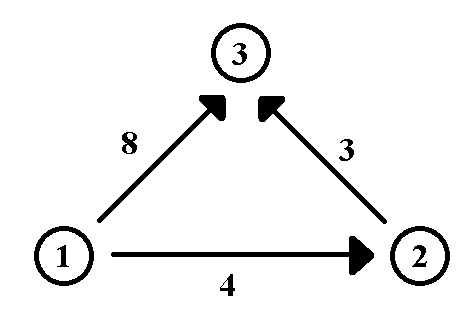
\includegraphics{./images/dijkstra_priklad.png}}
  \caption{Orientovaný graf s ohodnotenými hranami}
  \label{dijkstra_priklad}
\end{figure}

Priebeh dijkstrovho algoritmu vysvetlíme na jednoduchom príklade. Máme orientovaný graf ako je zobrazený na obrázku~\ref{dijkstra_priklad}. Našou úlohou je nájsť najkratšiu cestu z vrcholu $1$ do ostatných vrcholov. Učiníme tak teda zapomoci dijkstrovho algoritmu. Čiže, najprv si vytvoríme pole, označme ho $D$, v ktorom si pre každý vrchol budeme pamätať hodnotu doň najkratšej cesty z vrcholu $1$. Na počiatku bude táto hodnota pre všetky vrhcoly nekonečno, respektíve nejaká jeho rozumná náhrada. My budeme používať nekonečno. Nastavíme $D [1] = 0$. Začíname teda s počiatočným vrcholom $1$. Zoberieme jeho všetkých zatiaľ nenavštívených susedov (vrcholy $2$ a $3$), a porovnáme hodnoty takto: najprv pre vrchol $2$, zistíme či je jeho hodnota v poli $D$ (to jest nekonečno) menšia ako hodnota vrchola, z ktorého vychádzame, plus hodnota hrany (to jest 0 + 4). To ale nie je pravda, takže prepíšeme hodnotu $D [2]$ na $4$. Pre vrchol $3$ zasa porovnávame nekonečno s hodnotou $0+8$ alebo aj, ako je v algoritme~\ref{Alg_Dijkstra} naznačené, minimum z týchto dvoch hodnôt zapíšeme do $D [3]$. Vrchol $1$ nemá viac susedov, takže ho označíme ako navštívený a pokročíme. Ďalším vrcholom v poradí bude ten s najmenšou hodnotou $D [i]$ spomedzi doposiaľ nenavštívených, čiže vrchol $2$. Ten má iba jedného ešte nenavštíveného suseda, a to vrchol $3$. Do $D [2]$ preto zapíšeme minimum z hodnôt $8$ a $4 + 3$. Vrchol $2$ je týmto vybavený a označený za navštívený. Zostáva posledný vrchol - vrchol $3$. Väčšina implementácií dijkstrovho algoritmu pri dosiahnutý finálneho vrcholu končí v snahe urýchliť vyhľadávanie medzi dvoma vrcholmi. Ak vśak túto podmienku nezakomponujeme do nášho algoritmu, program zráta hodnoty najkratších ciest z daného vrcholu do všetkých ostatných vrcholov. V našom prípade nie je veľmi podstatné, ktorú variantu zvolíme, keďže algoritmus tak či tak vo vrchole $3$ skončí, nakoľko ten už nemá žiadne incidentné hrany a v grafe už nejestvujú ďalšie nenavštívené vrcholy. Dosiahli sme teda výsledok: najkratšie cesty z vrcholu $1$ sú uložené v poli $D$. Najkratšia cesta do vrcholu $1$ je $D [1] = 0$, do vrcholu $2$ je $D [2] = 4$ a pre vrchol $3$ je odpoveď $D [3] = 7$.\newline

Týmto príkladom sme chceli jemne ozrejmiť postup pracovania algoritmu, keďže pre tých, čo sa s ním ešte nestretli, ho môže byť dosť obtiažne z pseudokódu~\ref{Alg_Dijkstra} vybadať.\newline

Keďže je našim cieľom nie ani tak zistiť cenu najlacnejšej cesty, čo je hlavnou úlohou popísaného algoritmu, ale skôr takéto cesty nájsť, dijkstrov algoritmus by sme potrebovali jemne modifikovať, a to tak, aby sme vedeli spätne zrekonštruovať nájdené cesty. Teda so znalosťou konečného vrchola by sme chceli vedieť vygenerovať postupnosť vrcholov, cez ktoré sme sa do finálneho vrchola dostali. Budeme si preto pamätať pri každom vrchole informáciu, z ktorého vrchola sme sa doň dostali.\newline

Dijkstrov algoritmus sa zdá byť najvhodnejším kandidátom pre účely našej práce. Jeho časová zložitosť je príjemná, implementácia nenánorčná a je dosť ľahké sa v nej orientovať, takže si ju budeme môcť poľahky modifikovať, prispôsobiť našim potrebám. Budeme teda schopný vypísať dodatočné informácie pre používaťeľov aplikácie, prípadne vyhľadávanie spresniť či rozšíriť podľa ich potrieb.\newline


\subsection{Bellman\textendash Fordov algoritmus}

Ďalším algoritmom na výpočet najlacnejších ciest v grafe je Bellman\textendash Frodov algoritmus. Hoci ako prvý prišiel s týmto riešením Alfonso Shimbel v roku 1955, algoritmus bol pomenovaný po Fordovi, ktorý ho publikoval v roku 1956 a po Bellmanovi, ktorého publikácia je z roku 1958. Ten istý algoritmus zverejnil i Moore v roku 1957, a preto niekedy môžeme počuť aj o Bellman\textendash Ford\textendash Moorovom algoritme.\newline

Samotný algoritmus, narozdiel od dijkstrovho, dokáže pracovať i so záporne ohodnotenými hranami. Avšak predpokladá sa, že graf neobsahuje záporne cykly, to jest cykly, ktorých celková cena má zápornú hodnotu. Ak by v grafe existoval aspoň jeden, mohli by sme po ňom prejsť ľubovoľne veľa krát, čím by sme ustavične znížovali najlacnejšiu cenu do viacerých vrcholov. Bellman\textendash Fordov algoritmus je však navrhnutý tak, že zakaždým vykoná konečný počet krokov, takže i pri grafe obsahujúcom záporný cyklus skončí, nezacyklí sa, iba jeho výsledné hodnoty nebudú pravdivé. Navyše, mnohé implementácie zahŕňajú i detekciu takéhoto cyklu a pri jeho nájdení vyhlásia chybu. Naša implementácia takúto kontrolu obsahovať nebude, nakoľko nie je potrebná pre vysvetlenie funkcionality a fungovanie algoritmu.\newline

Náš algoritmus predpokladá, že na vstupe dostane graf $G = (V, E)$ neobsahujúci záporné cykly, hodnotiacu funkciu $h: V \times V \rightarrow R$ a počiatočný vrchol $v_{0}$. Ďalšie predpoklady sú, ako u dijkstru, že ak $uv \notin E$, potom $h(u,v) = \infty$, taktiež $h(u,u) = 0$ a napokon, že funkciu $h$ je možné vypočítať v čase $O(1)$. Aby sa nám ľahšie pracovalo, opäť povedzme, že vrcholy na vstupe musia byť reprezentované celými číslami $1, 2, ... , n$, kde $n$ je počet vrcholov grafu. Našim výsledkom bude pole čísel $D$, v ktorom bude pre každý vrchol $v \in V$ vypočítaná cena najlacnejšej cesty z počiatočného vrchola $v_{0}$ do $v$, ozačená $D [v]$. Nasledovná implementácia je zostavená s pomocou knihy od Bannistera a Eppsteina \cite{bannister2012randomized}.\newline

\begin{algorithm}[H]
  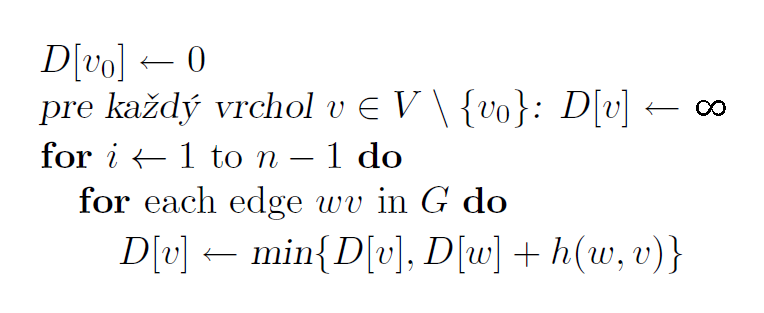
\includegraphics[width=\linewidth]{./images/Alg_Bellman-Ford.png}
  \caption{Bellman\textendash Fordov algoritmus}
  \label{Alg_Bellman-Ford}
  \centering
\end{algorithm}

Časová zložitosť algoritmu je očividne $O(|V|\cdot |E|)$. Jeho korektnosť je možné nájsť napríklad v knihe \cite[kapitola 3.3.4]{bang2008digraphs}. Toto dielo navyše obsahuje aj implementáciu spomínaného drobného vylepšenia, a to zisťovanie prítomnosti záporného cyklu.\newline

\begin{figure}[H]
  \centering{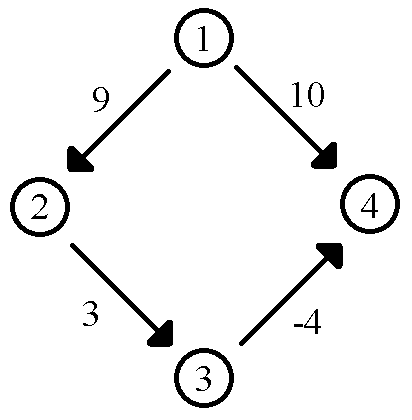
\includegraphics{./images/bellman-ford_priklad.png}}
  \caption{Orientovaný graf s ohodnotenými hranami}
  \label{bellman-ford_priklad}
\end{figure}

Funkcionalitu algoritmu si opäť predvedieme na jednoduchom príklade. Nech je vstupným grafom algoritmu graf vyobrazený na obrázku~\ref{bellman-ford_priklad}. Naším cieľom bude nájsť najkratšiu cestu z vrcholu $1$ do ostatných vrcholov. Pod týmto popisom sa nachádza aj tabuľka (tabuľka~\ref{priebeh_bellman-ford}) ukazujúca kľúčové hodnoty počas vykonávania algoritmu na našom príklade. Iterácia číslo 0 zaznamenáva stav vrcholov po inicializácií a pred začatím vykonávania cyklu, preto má počiatočný vrchol v tomto momente hodnotu $D [1] = 0$ a všetky ostatné $D [j] = \infty$. Počas iterácie $i = 1$ sa ideme pozerať na všetky hrany v grafe. Tu zavisí od ich usporiadania, ktorá z nich sa vezme v akom poradí. V našom príklade, aby sme demonštrovali čo najviac možností, povedzme, že ako prvú určíme na porovnávanie hranu medzi vrcholmi $2$ a $3$. Keďže je ale hodnota $D[2]$ aj $D[3]$ rovná nekonečnu, zapíšeme do $D[3]$ opäť nekonečno. Nech je ďalšou hranou v poradí vyhodnocovania hrana medzi vrcholmi $1$ a $2$. Tu je už situácia príznačnejšia. Nakoľko poznáme hodnotu $D[1]$, môžeme zaznačiť, že $D[2] = 9$. Pozorné oko si isto všimne, čo by sa stalo, ak by boli vyhodnocovania týchto dvoch hrán v opačnom poradí. Totiž, v takom prípade by sme ihneď vedeli vypočitať i hodnotu $D[3]$. Pokračujme hranou medzi vrcholmi $1$ a $4$. Zisťujeme, že $D[4] = 10$. Hrana medzi vrcholmi $3$ a $4$ dovŕši prvú iteráciu algortmu. Tu sa ale nič nezmení, keďže porovnávame nekonečno s hodnotou $10$. V nasledujúcej iterácií $i = 2$ sa pre hrany spájajúce vrcholy $1, 2$ a $1, 4$ nestane nič zaujímavé. Pozrime sa teda na zvyšné hrany. Pre hranu medzi vrcholmi $2$ a $3$ sa upraví hodnota $D[3]$ na $12$ a následne sa pre poslednú hranu (medzi vrcholmi $3$ a $4$) vykoná porovnanie hodnôt ($D[4] = 10$) a $((D[3] = 12) + (-4))$. Po druhej iterácií sme už dospeli k optimálnemu riešeniu, čo ale náš algoritmus nemôže vedieť, a preto vykoná i poslednú, tretiu iteráciu. V nej sa ale už nič nezmení. Ak v dvoch stavoch po sebe nastala rovnaká situácia, repsektíve neprišlo k žiadnej zmene, je jasné, že algoritmus dosiahol výsledok. Ak by teda bola na pláne ešte ďalšia iterácia či nebodaj viac, môžeme vykonávanie programu ukončiť bez strachu pre nesprávny výsledok. Mnohé implementácie sú preto väčšinou doplnené o toto jemné vylepšenie. V našom príklade by nám však nepomohlo, keďže by program tak či tak zastavil po tretej iterácií.\newline

\begin{table}[H]
  \begin{center}
    \caption{Priebeh algoritmu}
    \label{priebeh_bellman-ford}
    \begin{tabular}{ | c | c | c | c | c | }
      \hline
      iterácia = i & D[1] & D[2] & D[3] & D[4] \\
      \hline
      0 & 0 & $\infty$ & $\infty$ & $\infty$ \\
      1 & 0 & 9 & $\infty$ & 10 \\
      2 & 0 & 9 & 12 & 8 \\
      3 & 0 & 9 & 12 & 8 \\
      \hline
    \end{tabular}
  \end{center}
\end{table}

V prípade Bellman\textendash Fordovho algoritmu je nám opäť na obtiaž jeho strohá funkcionalita, a teda zisťovanie cien najlacnejších ciest, zatiaľ čo my žiadame poznať celú nájdenú cestu. Modifikácia kódu je ale jednoduchá, rovnaká ako pre dijkstru - pre kaźdý vrchol si navyše zapamätáme, z ktorého vrcholu sme sa doň dostali.\newline

Bellman\textendash Fordov algoritmus má mnoho pozitív - aplikovateľnosť i na hrany so záporným ohodnotením. Jeho časová zložitosť je taktiež potešujúca a implementácia prehľadná. Avšak jeho funkčnosť i nad zápornými ohodnoteniami nám nijako nepomôže pri jeho aplikácií na grafikon hromadnej dopravy. Navyše, jeho časová zložitosť $O(|V|\cdot |E|)$ bude pri riešení nášho problému iba príťažou, nakoľko predpokladáme, že sieť liniek MHD bude obsahovať veľké množstvo hrán. Netreba však zabúdať, že algoritmus je pri iných problémoch široko využiteľný a výborný pre dobre zvolené dátové štruktúry.\newline


\subsection{Floyd\textendash Warshallov algoritmus}

Posledným algortimom slúžiaci na hľadanie najlacnejších ceist, ktorý uvedieme, nesie názov Floyd\textendash Warshallov algoritmus. Opäť, ako v predošlom prípade, sa ale ani Floyd, ani Warshall nemôžu pýšiť prvenstvom. Predbehol ich Roy publikáciou z roku 1959, zatiaľ čo Floydova i Warshallova boli obe z roku 1962. Warshall dokonca v jeho práci nadväzuje na Kleeneho algoritmus z roku 1956. Finálna verzia, ktorú aj mi predvedieme, dostala svoju podobu až na konci roku 1962 zásluhou Ingermana. Vďaka mnohým publikáciám sa tento algoritmus nazýva rôznymi menami. My si ale vystačíme s jedným.

Výsledok Floyd\textendash Warshallovho algoritmu sa značne odlišuje od predošlých dvoch. Zatiaľ čo tie spoľahlivo zistili hodnoty najlacnejších ciest z daného vrcholu do všetkých ostatných vrcholov, Floyd\textendash Warshallov ich vyráta z každého vrcholu do každého. Samozrejme, to by sme vedeli dosiahnuť aj použitím predošlých algoritmov na všetkych vrcholoch. Vyžadovalo by sa však mnoho réžie navyše a kód by sa pravepodobne priveľmi zneprehľadnil. Naopak, Floyd\textendash Warshallov algoritmus je na pohľad až príliš jednoduchý, no nesmierne účinný.

Nami uvedená implementácia bude pracovať s maticami. Na vstupe dostane algoritmus graf $G = (V, E)$ bez záporných cyklov a incidenčnú maticu $W = (w_{ij})$ rozmerov $|V|\times |V|$. Maticu $W$ si vieme jednoducho zostrojiť z hodnotiacej funkcie takto: Nech sú ceny hrán hodnotené hodnotiacou funkciou $h: V \times V \rightarrow R$, kde, ako obvykle, $h(u,u) = 0$, $uv \notin E \implies h(u,v) = \infty$ a $h(u,v) \in O(1)$. Potom $w_{ij} = h(i,j)$ pre všetky $i, j$. Príklad takejto matice $W$ je vyobrazený na \ref{C0}. Výsledkom algoritmu je posledná matica, a tou je matica $C^{(|V|)}$.\newline

\begin{algorithm}[H]
  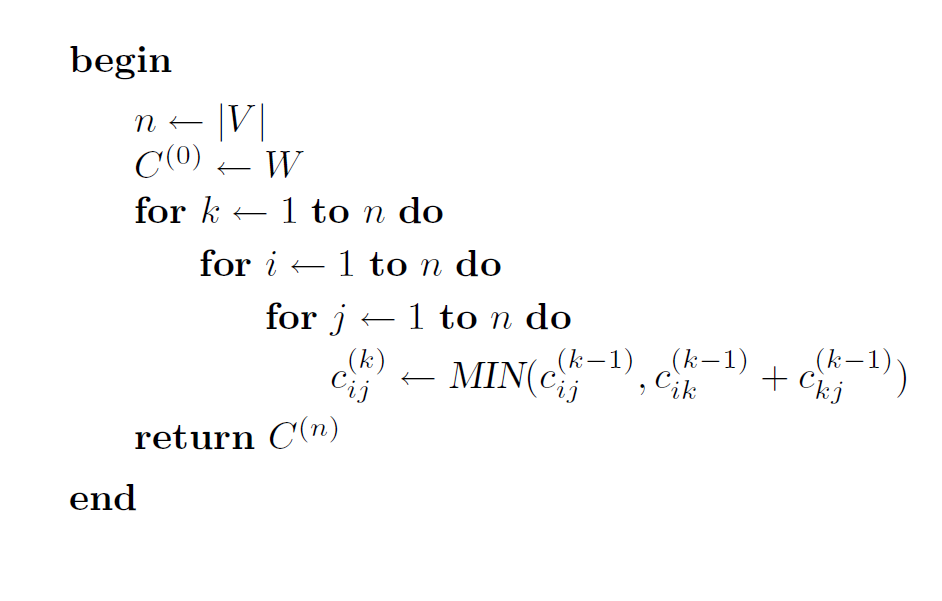
\includegraphics[width=\linewidth]{./images/Alg_Floyd-Warshall.png}
  \caption{Floyd\textendash Washallov algoritmus}
  \label{Alg_Floyd-Warshall}
  \centering
\end{algorithm}

Ľahko nahliadnuť, že časová zložitosť Floyd\textendash Warshallovho algoritmu je $O(|V|^{3})$. Jeho korektnosť je taktiež pohľadom badateľná. Pre istotu pridávame možnosť overiť si naše tvrdenie v knihe od Pavla Ďuriša, odkiaľ pochádza aj implementácia algoritmu \cite[kapitola 2.2.2]{duris2009}.\newline

\begin{figure}[H]
  \centering{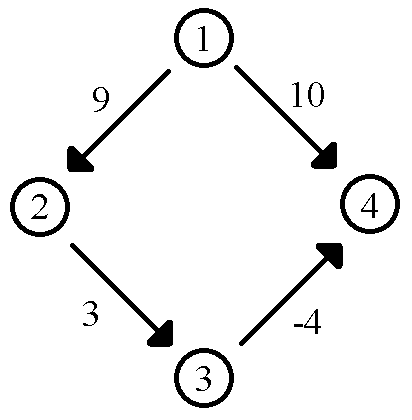
\includegraphics{./images/floyd-washall_priklad.png}}
  \caption{Orientovaný graf s ohodnotenými hranami}
  \label{floyd-washall_priklad}
\end{figure}

Ako príklad nám poslúži ten istý graf ako v prípade Bellman\textendash Fordovho algoritmu. Avšak výpočet algoritmu by bol na popis pridlhý, preto uvedieme iba zopár vyhodnocovaní a zaujímavé idey, ktoré je vhodné si uvedomiť. Prvý cyklus algoritmu, pracujúci s premennou $k$, vytvorí zakaždým celú novú maticu $C^{(k)}$. Pre každý riadok a stĺpec (premenné $i$ a $j$)  tejto novovznikajúcej matice sa vykoná porovnanie, ktoré vypočíta hodnotu momentálneho prvku. Napríklad, ak by sme chceli zrátať hodnotu v matici $C^{(1)}$ na pozícií $i = 2, j = 2$, s ľahkosťou využijeme vzorec použitý v algoritme, a teda $c^{(1)}_{2,2} = MIN (c^{(0)}_{2,2}, c^{(0)}_{2,1} + c^{(0)}_{1,2})$, po dosadení $c^{(1)}_{2,2} = MIN (0, \infty + 9) = 0$. Lepším príkladom môže byť zmena hodnoty v po sebe nasledujúcich maticiach, ako napríklad $c^{(3)}_{2,4} = MIN (c^{(2)}_{2,4}, c^{(2)}_{2,3} + c^{(2)}_{3,4}) = MIN (\infty, 3 + (-4)) = -1$.\newline

\begin{equation}
  \label{C0}
  C^{(0)} = W =
  \begin{pmatrix}
    0 & 9 & \infty & 10 \\
    \infty & 0 & 3 & \infty \\
    \infty & \infty & 0 & -4 \\
    \infty & \infty & \infty & 0
  \end{pmatrix}
\end{equation}

\begin{equation}
  \label{C1}
  C^{(1)} =
  \begin{pmatrix}
    0 & 9 & \infty & 10 \\
    \infty & 0 & 3 & \infty \\
    \infty & \infty & 0 & -4 \\
    \infty & \infty & \infty & 0
  \end{pmatrix}
\end{equation}

\begin{equation}
  \label{C2}
  C^{(2)} =
  \begin{pmatrix}
    0 & 9 & 12 & 10 \\
    \infty & 0 & 3 & \infty \\
    \infty & \infty & 0 & -4 \\
    \infty & \infty & \infty & 0
  \end{pmatrix}
\end{equation}

\begin{equation}
  \label{C3}
  C^{(3)} =
  \begin{pmatrix}
    0 & 9 & 12 & 8 \\
    \infty & 0 & 3 & -1 \\
    \infty & \infty & 0 & -4 \\
    \infty & \infty & \infty & 0
  \end{pmatrix}
\end{equation}

\begin{equation}
  \label{C4}
  C^{(4)} =
  \begin{pmatrix}
    0 & 9 & 12 & 8 \\
    \infty & 0 & 3 & -1 \\
    \infty & \infty & 0 & -4 \\
    \infty & \infty & \infty & 0
  \end{pmatrix}
\end{equation}

Opäť je namieste podotknúť, že nami požadované vylepšenie na poznanie i predchodcov s cieľom rekonštrukcie nájdených najlacnejších ciest treba pridať ešte ďalších $|V|$ matíc, ktoré si danú informáciu budú počas výpočtu ukladať. Ich definíciu je možné uzrieť v už menovanom zdroji \cite[kapitola 2.2.2]{duris2009}.\newline

Taktiež je vhodné poznamenať, že pre väčšie vstupy má algoritmus potenciál skonzumovať príliš veľa pamäte. Preto je v takom prípade výhodné algoritmus upraviť tak, aby používal iba dve matice, nakoľko pri algoritme je potrebné držať referenciu len na momentálnu a predchádzajúcu maticu ($C^{(k)}$ a $C^{(k-1)}$). To isté možno tvrdiť aj o maticiach predchodcov.\newline

Floyd\textendash Warshallov algoritmus je taktiež dobrým kandidátom pre riešenie nášho problému. Implementácia je opäť jednoduchá, časová zložitosť vítaná. Znovu ale, možnosť využitia algoritmu i na záporných hranách nie je pre nás nijako prínosná. Naviac, pri vyhľadávaní spojenia medzi dvomi zastávkami v grafikone MHD by bolo nutné vyrátať hodnoty najlacnejších ciest z každého vrcholu do všetkých vrcholov, čo môže trvať prdlho. Samozrejme, po skončení hľadania budú už nasledujúce dopyty uspokojené v konštantnom, resp. lineárnom (ak uvažujeme i rekonštrukcie ciest), čase.\newline


\subsection{Zhrnutie}
\label{vyhlad_alg_zhrnutie}

Všetky tri prezentované algoritmy sú vhodnými adeptami pri riešení problému vyhľadávaní spojení v grafikone MHD. Kaźdý z nich má svoje pozitíva, ale i nedostatky. Ktorí z algoritmov bude najvhodnejší, zavisí hlavne od dát, nad ktorými bude pracovať. Ako sme už spomínali, Bellman\textendash Fordov algoritmus bude mať výhodu pri grafoch obsahujúcimi menšie množstvo hrán, čo, žiaľ, nebude prípad liniek MHD. Floyd\textendash Warshallov algoritmus je zasa zostavený tak, aby vypočítal všetky najlacnejšie cesty. Preto bude jeho priebeh pri väčšich vstupoch neprimerane dlhý. Jeho využitie preto vidíme pri grafikonom MHD malých miest, kde sa vyrátajú vsetky potrebné hodnoty už pri inicializácií, najlepšie na druhom vlákne, aby mohol používateľ zadávať dopyt už počas výpočtu. Využitie algoritmu by bolo v tomto prípade priam žiadané, keďže ostatné dva algoritmy môžu svoje výpočty pri väčšine postupností dopytov opakovať, čo ich môže nažiadane zdržovať. A nakoniec, Dijkstrov algoritmus sa zdá byť najvšeobecnejší a najpoužiteľnejší pre ľubovoľné dáta.\newline

Existujú aj iné, pokročilejšie algoritmy, ktoré sú schopné nájsť najlacejšie cesty v grafe. Zvyčajne však ide o kombináciu nami uvedených algoritmov, prípadne ich optimalizácia alebo nejaká rafinovaná modifikácia. Na predstavu poslúži Johnsonov algoritmus, ktorého výstup je rovnaký ako výsledok Floyd\textendash Warshallovho algoritmu, len jeho priebeh je iný - využíva kombináciu Dijkstrovho a Bellman\textendash Fordovho algoritmu, čím dosahuje na riedkych grafoch výsledok rýchlejšie. Spomínaným pokročilejším algoritmom sa však podrobnejšie v našej práci venovať nebudeme.\newline

